\section*{Experimental Results}

The dataset used for the experiments is the famous \emph{Recipes1M+} \cite{15}, a collection 
created by MIT, consisting of more than one million culinary recipes. 
Of all these recipes, only a subset of 51235 documents of it was used due 
to their informative content which best fits the purpose of this study. The 
information about the line distributions for each recipe indicates that the 
instruction field contains a higher number than the information contained in 
the ingredients field. To have good performance in finding, we preferred to 
choose the "instructions" field (\ref{distributions}). The first ranking of relevant documents, 
generated by the tf-idf method, was evaluated following two different 
approaches that could best be linked with the principle explained in \cite{16}. 
Specifically, each category of a recipe is considered as an entity associated 
with a document. Both approaches rely on being able to compare the categories of relevant documents 
with the category of the target document. Since the categories are not present in the dataset, the 
two proposed approaches deal with being able to "extract" these categories directly from the web. 
\begin{figure}[h!]
    \centering
    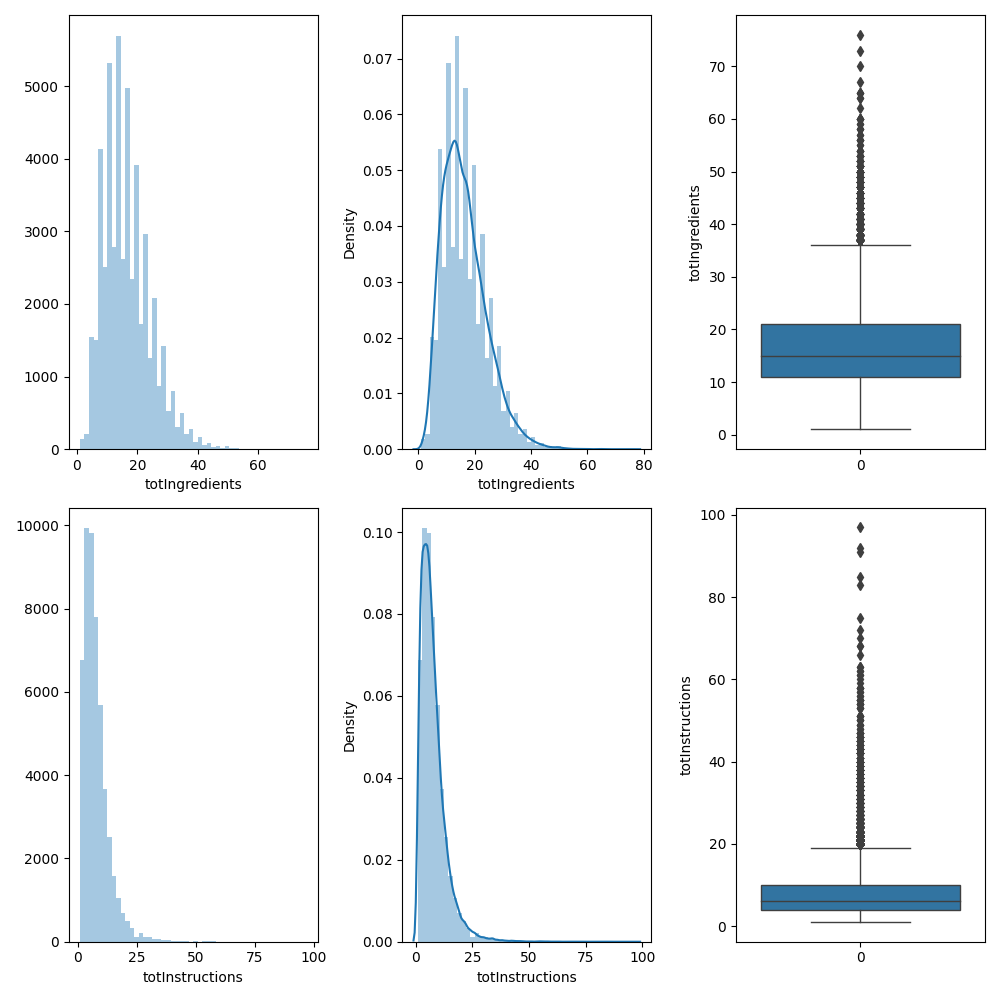
\includegraphics[width = 0.7 \linewidth]{images/displot.png}
    \centering
    \caption{Distributions of lines per ingredients and instructions.}
    \label{distributions}
\end{figure}
The first approach uses an API, called \href{https://pypi.org/project/scrape-schema-recipe/}{\emph{Scrape Schema Recipe}}, 
which takes the link associated with the recipe website, present in the dataset, and scrapes the corresponding category.
Unfortunately not all the links are still existing, therefore the evaluation of the ranking takes place following three types of methods:
\begin{enumerate}
    \item {\bfseries Overestimated}: consider the uncategorized document as good;
    \item {\bfseries Underestimated}: considers the uncategorized document not good;
    \item {\bfseries Discarded}: Discard the uncategorized document from the evaluation.
\end{enumerate}
As for the second method, this makes use of the \href{https://fdc.nal.usda.gov/api-guide.html}{\emph{USDA}} API, a library that has the task 
of taking every single ingredient of the recipe and fetching the corresponding category from a large database belonging to the United States 
Department of Agriculture. Compared to the first approach, the recipes that did not have a category are only four recipes. It is worth mentioning 
that both approaches are computationally expensive as the extraction of all categories took about two days. In addition to all these evaluations, 
it was decided to create a last one derived from a mixed approach (Scrape + USDA). Taking five random queries, the evaluations of the corresponding 
rankings are those reported in table (\ref{avgp}).
\begin{table}[h!]
    \centering
    \begin{adjustbox}{max width=\textwidth}
    \begin{tabular}{|c||c|c|c||c||c||}
        \hline
        \multirow{2}{*}{\bfseries{Queries}} & \multicolumn{3}{c||}{\bfseries{Scrape Schema Recipe}} & \multicolumn{1}{c||}{\bfseries{USDA}} & \multicolumn{1}{c||}{\bfseries{Mixed (Scrape+USDA)}} \\            & \bfseries{Overestimate} & \bfseries{Underestimate} & \bfseries{Discarded} & \bfseries{}  & \bfseries{}\\
        \hline
        \hline
        \RN{1} & 0.7520 & 0.3734 & 0.5958 & 0.9817 & 0.9947\\
        \hline
        \RN{2} & 0.9309 & 0.6780 & 0.9054 & 1.0 & 1.0\\
        \hline 
        \RN{3} & 0.7458 & 0.2746 & 0.5411 & 0.9797 & 0.9982\\
        \hline
        \RN{4} & 0.8939 &  0.5320 & 0.8433 & 0.9612 & 0.9870\\
        \hline
        \RN{5} & 0.8335 & 0.5033 & 0.7544 & 0.9940 & 0.9940\\
        \hline
        \hline
        Average & 0.8312 & 0.4722 & 0.7280 & 0.9833 &  \bfseries 0.99478 \\
        \hline
    \end{tabular}
    \end{adjustbox}
    \caption{Average Precision on each query for each method.}
    \label{avgp}
\end{table}
As you can see, the mixed approach is the one that, in terms of average precision, manages to achieve the best evaluation.
Moving on to the evaluation of the new queries generated, a visual comparison, based on a PCA, was used between the ranking 
generated by the tf-idf method and each new query produced by the project core (\ref{PCA}). The goal is to find a query whose distance 
from the target document is less than all other distances produced by the remaining queries.
\begin{figure}[h!]
    \centering
    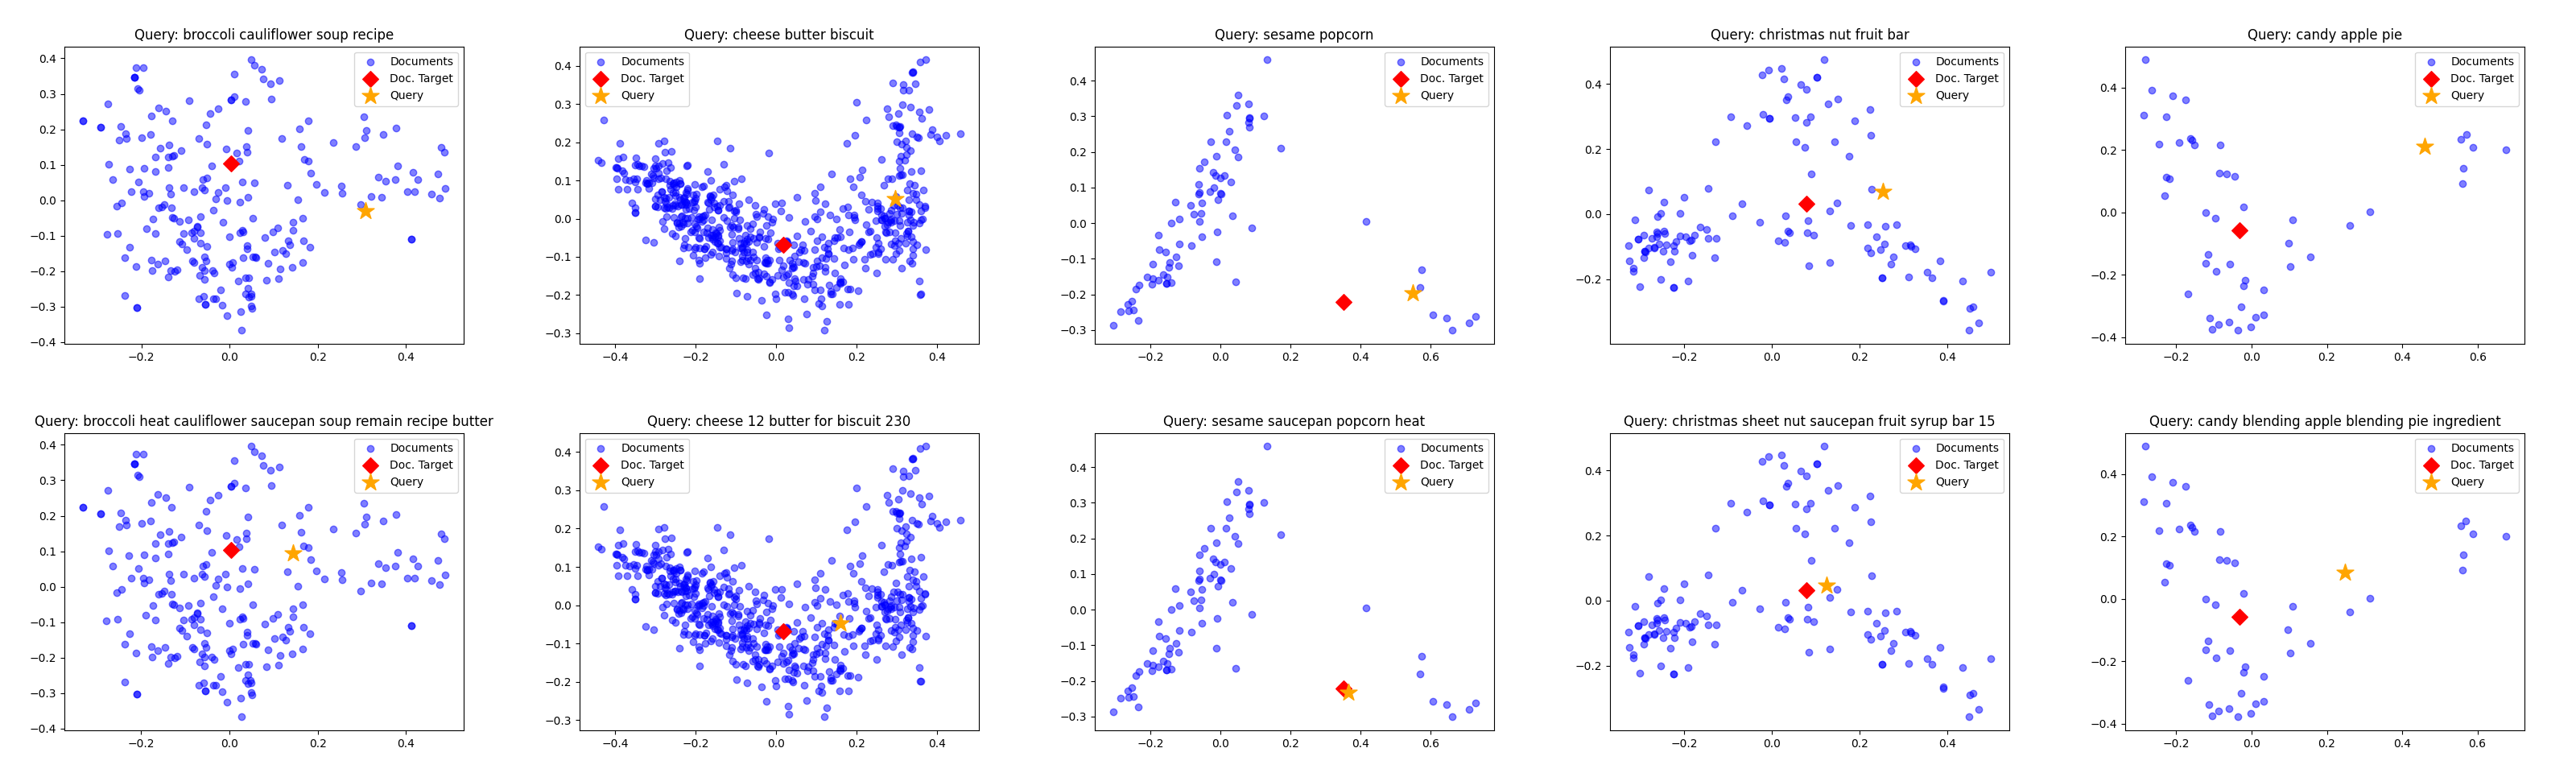
\includegraphics[width =\linewidth]{images/PCA paper/PCA all.png}
    \centering
    \caption{PCA initial query (top) and expansive query (bottom).}
    \label{PCA}
\end{figure}
